\section{The Gisele clinical pathway analyzer\label{section:tool-clinical-pathway-analyzer}}

A clinical pathway is a well-defined process, based on medical protocols, guidelines and recommendations; centered on a specific patient class with similar needs; involving a multi-disciplinary team; and addressing clear clinical goals \cite{Middleton:2000}. 

The tool presented in this section is motivated by a joint project aimed at building and analyzing models of clinical pathways. Guarded hMSCs have been chosen as the particular kind of process models, for which analyses discussed in \cite{Damas:2011} have been implemented. These analyses are actually made at the g-LTS level; the tool here thus relies on the synthesis algorithm from g-hMSC to g-LTS described in Section \ref{subsection:from-ghmsc-to-glts}.

A snapshot of the main screen of the tool is shown in Fig.~\ref{image:gisele-tool}. A guided tour of the tool on a medical case-study can be found in \cite{Damas:2011}. In this section, we will highlight keypoints of its implementation and discuss a few design decisions. The main features implemented in the tool are:

\begin{figure}
\centering\scalebox{.525}{
  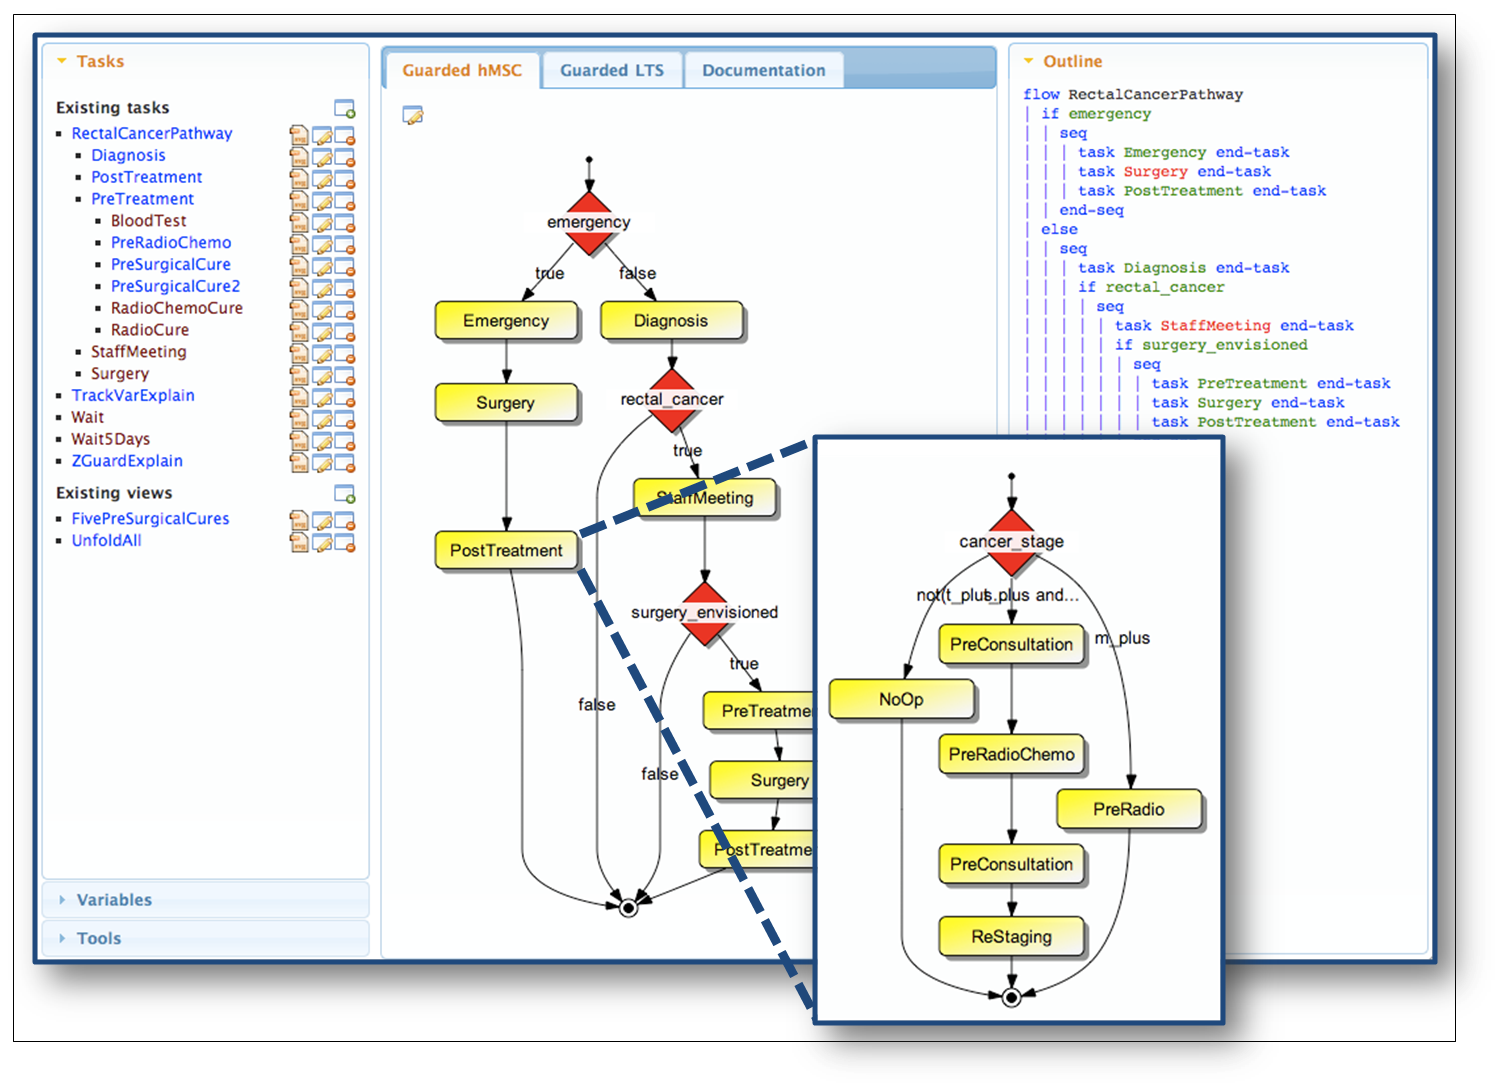
\includegraphics[trim=5mm 10mm 10mm 5mm, clip]{src/7-tool-support/images/gisele-tool}}
  \caption{The Gisele tool, a clinical pathway analyzer\label{image:gisele-tool}}
\end{figure}

\begin{itemize}
\item The modeling and visualization of process models made of tasks and decision nodes defined on fluents (see Section \ref{section:background-process-models}). Tasks can be successively refined in sub-processes, as illustrated in Fig.~\ref{image:gisele-tool}.
\item A variety of analyses for checking the completeness, non overlapping and accuracy of decision nodes; verifying pre-conditions of tasks; analyzing processes in terms of timing and dosage; and so on (see \cite{Damas:2011}).
\item Dedicated screens for eliciting process models; documenting them with stakeholders; unfolding process models for specific analyses; projecting them on specific patient classes, and so on.
\end{itemize}

\subsection*{Architecture and design decisions}

The architecture of the tool is illustrated in Fig.~\ref{image:gisele-tool-architecture}. Its main modules are explained below in the light of our main design decisions.

\begin{figure}
\centering\scalebox{.5}{
  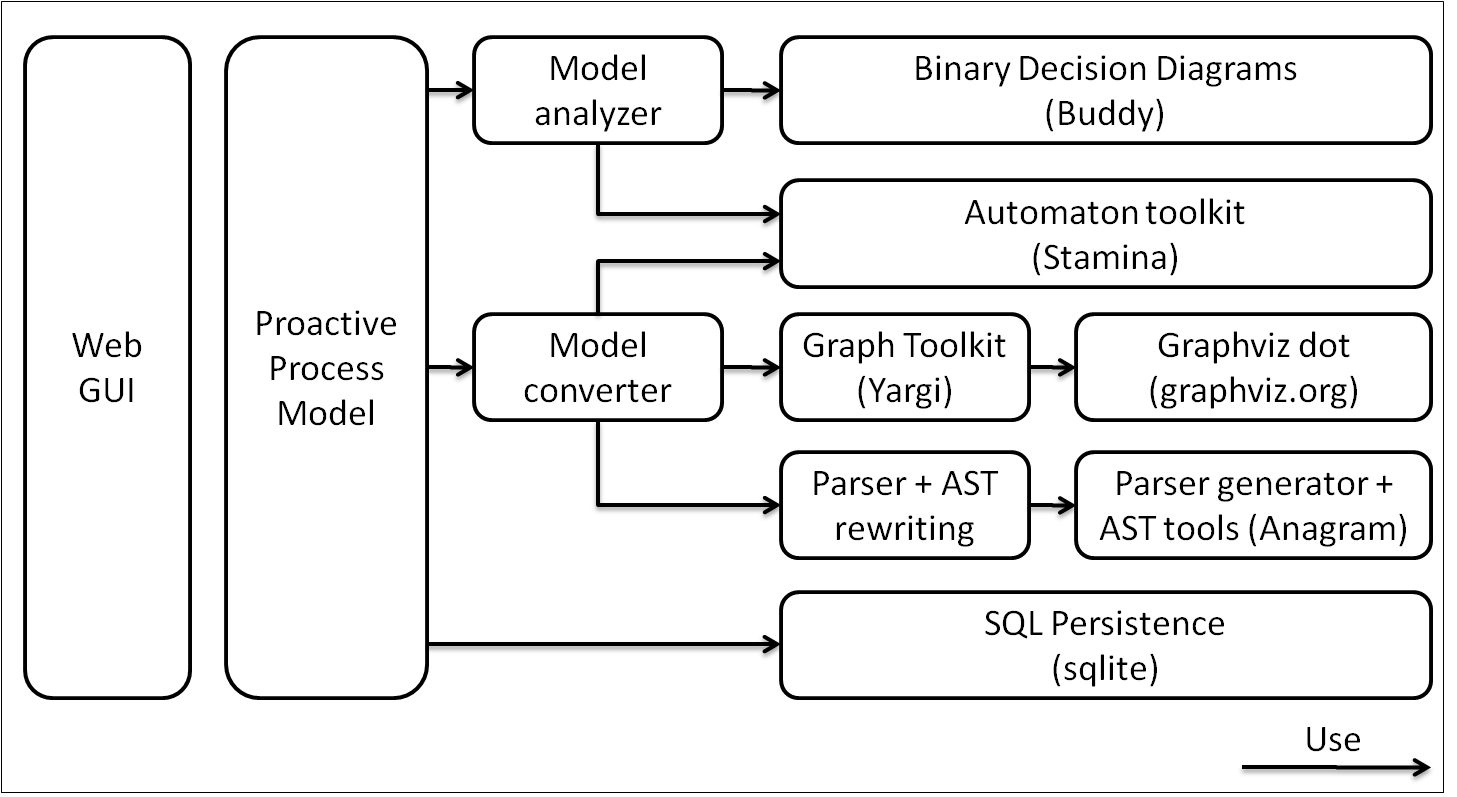
\includegraphics[trim=3mm 3mm 3mm 3mm, clip]{src/7-tool-support/images/gisele-tool-architecture}}
  \caption{Architecture of the Gisele tool\label{image:gisele-tool-architecture}}
\end{figure}

\begin{description}
\item[Process language] To keep the tool simple to use and to develop, a simple process language is used instead of a graphical process editor. This module defines a grammar and an API on top of parsing and abstract syntax tree rewriting tools of the \emph{anagram} library.

The process language uses common abstractions from structured programming, i.e. sequencing of tasks, if/then/else, guarded commands (case), while and until loops, and so on. However, it keeps the semantics of guards and variables abstract; in other words, fluent definitions are not constructions of the process language itself.

For example, the meeting scheduling process can be translated to this process language as show in Fig.~\ref{image:meeting-scheduling-gis}.

\begin{figure}
\centering\scalebox{1.0}{
  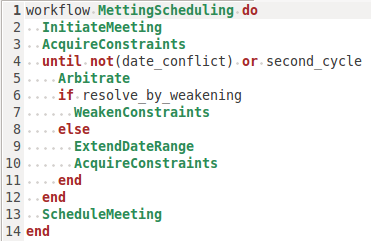
\includegraphics[trim=0mm 0mm 0mm 0mm, clip]{src/7-tool-support/images/meeting-scheduling-gis}}
  \caption{Meeting scheduling process encoded in the Gisele tool\label{image:meeting-scheduling-gis}}
\end{figure}

\item[Rich pathway model] In addition to process definitions, a complete pathway model is composed of several tasks in successive refinements, fluent definitions, task documentation, and so on. This structural module implements a rich model for clinical pathways; such pathways are kept persistent with the use of the SQLite database engine.

The implementation of a \emph{rich} model is an important design decision of the Gisele tool. Roughly, this pattern consists in seeing all analysis results as part of the pathway model instead of being computed ``from its outside''; the distinction between what is a base information and what is a a derived/computed one is kept secret by the module.

With such a pattern, displaying a process instance together with annotations about analysis results is seen a simple query. The module automatically triggers the analysis execution if needed to answer the query. 

We come back to this design decision in the discussion section later.

\item[Process rewriting] The implementation of the rich pathway model relies on specific algorithms for rewriting processes as multiple views. For example, a process instance is parsed and kept as an abstract syntax tree (AST); rewrited as a guarded hMSC for being displayed; compiled in an equivalent guarded LTS for analyses; and so on. 

Rewritings algorithms are implemented in the ``Process rewriting'' module, and rely on external libraries for parsing, rewriting ASTs, manipulating graphs and automata. This module also provides traceability support between the multiple views of the same process instance.

\item[Process analyzer] This module implements the process analyses discussed in \cite{Damas:2011}; they rely on different instantiations of an abstract fixpoint algorithm on g-LTS. Such analyses makes an intensive use of automata and binary decision diagrams with the help of dedicated libraries. 

For every process instance, the rich model automatically triggers the execution of an analyse as soon as its results are needed. Those results are kept as decoration of the g-LTS states. These decorated states are kept as an cache for analysis results. This cache is cleaned up when a process definition changes by simply throwing its g-LTS away.

\item[Web GUI] The last module is the graphical user interface (GUI), that mostly runs inside a web browser. Thanks to services offered by the rich model, the implementation of the GUI turns to a simple model navigator, implemented internaly with an MVC pattern. 

The main screen of this navigator is made of three panels (see Fig~\ref{image:gisele-tool}). 
\begin{itemize}
\item The left one gives a global outline of the clinical pathway and allows navigating it; links are provided to open and update task and fluent definitions.
\item The current task is always displayed as a process graph in the middle panel. The layout of the graph is automatically computed with the well-known \emph{dot} utility\footnote{available at http://graphviz.org}. Nodes of the graph can be clicked to navigate the model through task refinements.
\item The current task is also outlined through an annotated abstract syntax tree in the right panel. Annotations provide analysis feedback to the user: tasks and decision nodes for which at least one analysis fails are displayed in red; clicking on a node on this tree gives a detailed analysis explanation and counter-examples on analysis failures.
\end{itemize}

\end{description}

\subsubsection*{Discussion}

This rich model module and its use of the ``Process rewriting'' and ``Process analyzer'' is an important design decision of the Gisele tool. The idea is to make the opposite of the ISIS tool with respect to analyses and user feedback. 

In the ISIS tool, synthesis and analyses are made ``on demand'': for example, the user explicitely launches consistency checks and receives dedicated feedback as a result (see Section \ref{section:tool-support-isis}).

In the Gisele tool, the end-user navigates her model thanks to the GUI that runs inside a web browser. Everytime she looks at a task, the tree at right provides her with feedback about analyses and their results: green means success, red means fail. The pattern is inspired from continuous compilation chains in integrated development environments (IDE) such as Eclipse. 

Our experience with that pattern is that it provides a natural and effective user experience in terms of modeling and continuous improvement of a clinical pathway. However, the smoothness of the navigation might be slightly hurted because the execution of analyses is automatically triggered but may require time to finish. The current version of the tool freezes the GUI with a friendly waiting message. Other heuristics are worth considering, such as implementing a background execution of the analyses that are the most likely needed or deferring the display of specific parts of the UI.
